\chapter{Technologies and Methods}
\label{sec:tech_and_methods}
This chapter gives a quick introduction to the non-trivial technologies and methods used while developing the system. For purposes of brevity, technologies that are well known or only marginally relevant to the following chapters have been ommited\footnote{Such as CSS3, HTML5, JS ES6, CSS Preprocessors, the vue-router extension, and the Git distributed version control system}. The utilized technologies can roughly be categorized into runtime specific technologies, which are relevant during system execution, and development technologies, which are only relevant while developing, compiling, and testing the system. 
\section{Runtime specific Technologies}
\subsection{Vue.JS ecosystem}
\subsubsection{Vue Framework}
Vue is a Javascript framework used for simplifying the development of reusable, responsive frontend components. The core framework was initially developed by Evan You, in 2014. Since then, the framework quickly gained popularity in the open source community, currently being the 5th most popular open source project on the popular code sharing platform GitHub \cite{GitHubMostStars}. The framework serves a similar purpose as other popular Javascript frontend libraries such as React and Angular, though design, scope, and implementation differences can be found in various places \cite{VueComparisonOtherFrameworks}.
\subsubsection{VueX: State management and Flux Architecture}
The Vue core library is intentionally restricted in scope to the applications view layer. However, a vast Ecosystem has recently emerged around the Vue library covering other required functionalities of modern Web Applications, such as state management, client-side routing, or network connectivity. VueX is a library providing a state management system to the Vue core library which is modelled after Facebooks Flux Architecture \cite{Vuex}\cite{FacebookFlux}. It serves as a centralized store where all application state is located. State can only be retrieved and modified in a predictable fashion. This results in easier maintainability and extensibility for large applications, as developers always know how state is located, accessed, and modified.
\subsubsection{Material Design Components}
Material Design is an open source user interface design system developed and maintained by Google. It consists of design guidelines, components, and development tools. At the time of writing, it is being used in a large quantity of Google products. Furthermore, it is the officially recommended Design Language to use when developing Applications for the Android Platform \cite{AndroidAppQualityGuidelines}. The Design Components are thus familiar and intuitive to use for a large amount of potential end users. The Design Components are available for Vue.JS applications through the vue-material library \cite{VueMaterial}.
\subsection{Reactive Extensions and rx.js}
\gls{RX} is a language agnostic, open source API for asynchronous programming with observable streams. It can be seen as an extension of the Observer pattern \cite{ReactiveXManual}, one of the twenty-three well-known "Gang of Four" design patterns \cite{Gamma:1995:DPE:186897}.

The traditional Observer pattern is based on the fundamental concepts of the \emph{Observable} and the \emph{Observer}. The \emph{Observable} has the ability to \emph{emit} items over time. An \emph{Observer} may declare a dependency on the \emph{Observable} by means of \emph{subscribing} to it. If a subscription has been established, the \emph{Observer} will receive the items as they are emitted from the \emph{Observable}.

The \gls{RX} specification extends on this concept by providing a variety of \emph{Observable operators} to change the emission behavior, transform the emissions, or combine multiple \emph{Observables}.

\begin{figure}[h]
    \centering
    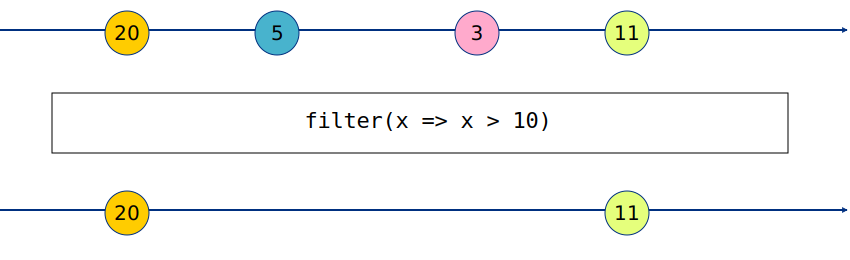
\includegraphics[width=10cm]{filter}
    \caption{An example Observable transformation, represented using \emph{Rx Marble Diagrams}.}
    \label{fig:rx-marbles-filter}
\end{figure}
%
Figure \ref{fig:rx-marbles-filter} gives a visual presentation of an Observable transformation. The top and bottom arrows both represent Observables. The arrow-direction represents time, the colored circles on the arrows represent items emitted by the Observable. The box in the center represents the application of an Observable operator, in this case the \emph{filter} operator, which filters Observable emissions by applying the given predicate, in this example $x > 10$. The result of the transformation is a new Observable that only includes the items that match the given predicate.

Apart from the Observable operators, \gls{RX} also includes specialized versions of the traditional Observable, such as the \emph{Subject}, which has the property of being able to act as Observable and Observer simultaneously, or the \emph{Single}, which represents a singular value emission in the future (similar to the Javascript ES5 Promise).


\subsection{Leap Motion Device}
\subsubsection{Virtualized Domain Model}
The Leap Motion Device is capable of producing a virtualized model of one or more hands placed inside the devices field of view. The Device Data consists of a stream of JSON-formatted device frames. Each device frame contains the current position of all detected hands in that point of time. The data is transmitted in a certain amount of \gls{FPS} (depending on device version, protocol version, and device driver settings), usually in the vicinity of $30 - 100$ \gls{FPS}.

\begin{figure}[h]
    \centering
    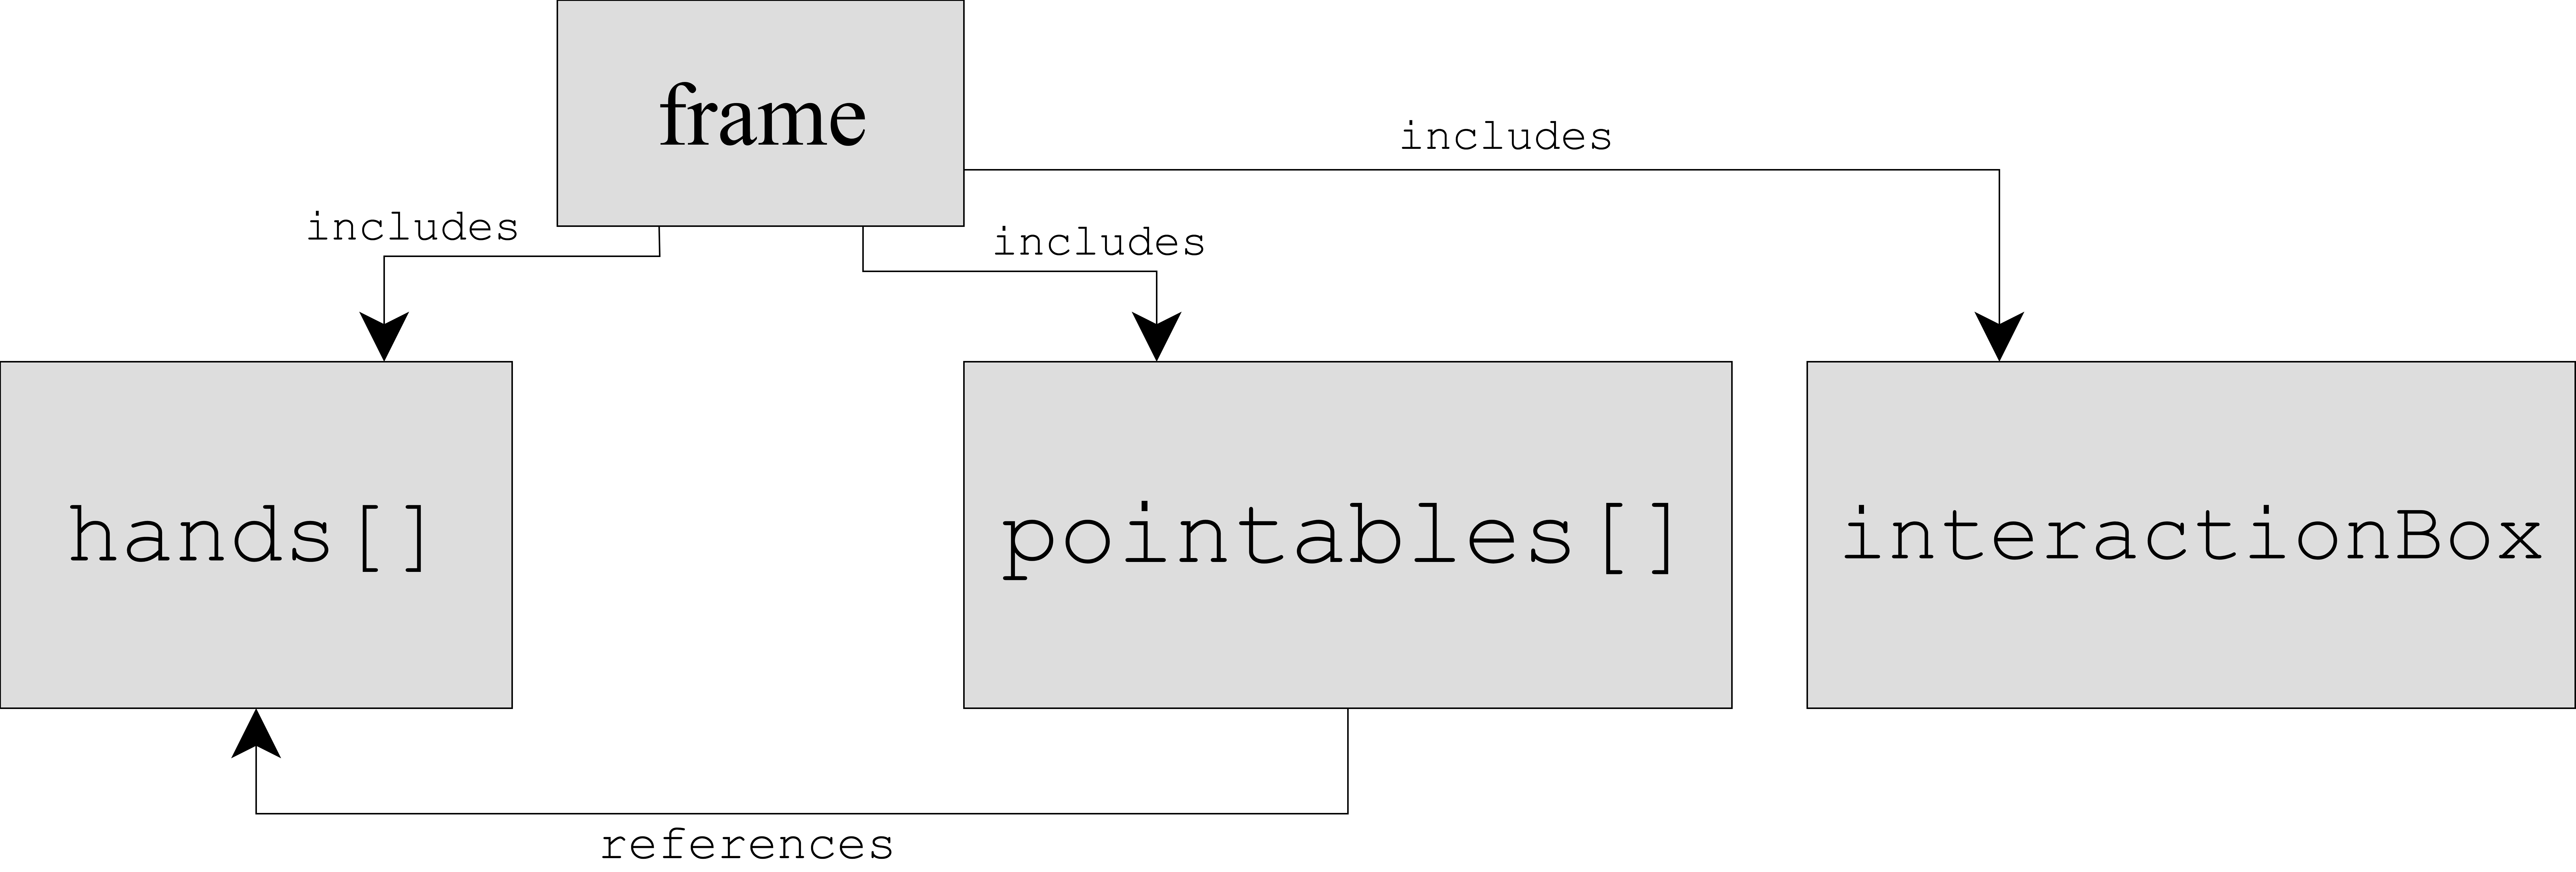
\includegraphics[width=8cm]{leap-data}
    \caption{High Level view of the Leap Motion Device Frame Data}
    \label{fig:leap-frame-data}
\end{figure}

Figure \ref{fig:leap-frame-data} gives an overview of the relevant device frame data. The frame data consists of multiple subcomponents. The subcomponents relevant for this paper are the \emph{hands} and \emph{pointable} arrays. The hands array contains representations of all hands that have been detected in the frame. The hand representations contain positional information, such as estimated position, width, and velocity, as well as metainformation, such as a frame-unique ID.

The pointables array essentially contains all detected fingers, though recent Leap Motion devices are capable of detecting other types of pointed objects as well. Like for tracked hands, positional information such as estimated position, width, velocity, and finger type (thumb, index..) is encoded in the representation. Additionally, recent Leap Motion Devices are capable of tracking skeletal information, such as the position of the hands metacarpals, proximal phalanges, intermediate phalanges, and distal phalanges \cite{LeapJsProtocol}. Finally, the pointable is associated to a hand by referencing its ID.

\subsubsection{Hardware Device Driver}
In order to interface with the Leap Motion Controller, its Hardware Device Driver has to be installed on the target device. The Hardware Device Driver is constituted by an operating system service named \emph{leapd} which interprets data coming from the Leap Motion controller and makes it available through a locally running Web Socket Server (see section \ref{sec:tech-web-sockets}).
\subsection{Graphics}
\subsubsection{THREE.js}
Recent Web Specifications such as WebGL make it possible to run graphically and computationally expensive programs directly in the browser, by allowing Web Applications to directly access the devices Graphical Processing Unit \cite[sec. 1]{WebGl2Spec}. Several Javascript libraries have since been created to simplify working with the WebGL API. A popular library is THREE.js, which is specializing simplifying the creation of 3D Applications.
\subsubsection{p5.js: Game Development}
p5.js is a simplistic Graphics Library similar in functionality to THREE.js. However, it primarily focused on 2D drawing, and has been simplified greatly in other aspects as well, allowing for rapid graphical prototyping and game development \cite{P5JS}.
\subsubsection{d3.js: Dynamic Documents and Visualizations}
The final relevant graphics library is d3.js, which greatly differs in purpose to the two previously introduced libraries. Its primary purpose is simplifying the creation of interactive, data-driven documents and data visualizations, such as diagrams and plots \cite[preface]{zhu2013data}. 
\subsection{Web Specifications}
\subsubsection{IndexedDB: Persistent Storage}
IndexedDB is a Browser API allowing the Browser Application to persist arbitrary data. It differs from other client side persistence APIs such as Cookies and Localstorage in various aspects, most notably the amount of data it can hold. Unlike Cookies and Localstorage, with both are constrained to a relatively small maximum size, the maximum size of an IndexedDB Database is usually much larger, sometimes restricted solely to the free space on an end devices hard drive\footnote{The exact size limitation depends on the implementation of the Web browser, as no standardization exists thus far.} \cite{MDNIndexedDB}. Additionally, IndexedDB allows for highly efficient storage access by providing the possibility to locate entries using incides. Though the exact implementation of the IndexedDB specification is dependent on the Browser vendor, it is usually implemented using a persistent B-tree data structure \cite[sec. 1]{IndexedDBSpec}.
\subsubsection{Web Workers: Javascript threading}
The Web Workers specification defines an API for executing Javascript code segregated from the main thread, often also called the window context. The Web Workers can thus be executed on a different processing core, resulting in no noticable performance inpact while navigating the Web Application, even if computationally expensive tasks are performed \cite[sec. 1.2.1]{workerdraft}. A Web Worker is able to communicate with the window context through a bidirectional, event based API \cite[sec. 4.6.1]{workerdraft}.
\subsubsection{Service Workers: Offline capability}
Service Workers are a special form of Web Workers that additionally allow the Web Application to work in an offline mode by means of intercepting and caching its asynchronous HTTP requests \cite[sec 4.5, 5]{serviceworkersdraft}.
\subsubsection{Web Sockets: bidirectional message streaming}
The WebSocket protocol is a protocol allowing for low overhead, full-duplex communication with a WebSocket compliant Server over a single TCP connection \cite[sec. 1.1]{rfc6455}. The protocol is able to be used from a Web Application context.
\label{sec:tech-web-sockets}
\section{Development specific Technologies}
\subsection{Webpack: module bundling}
\subsection{Typescript: static typing}
\subsection{Inversify: Inversion of Control}
\subsection{jest and sinon.js: Unit Testing and Mocking}